\usetikzlibrary{arrows,shapes,positioning,shadows,trees}



\tikzset{
  basic/.style  = {draw, text width=2cm, drop shadow, font=\sffamily, rectangle},
  root/.style   = {basic, rounded corners=2pt, thin, align=center,
                   fill=green!30},
  level 2/.style = {basic, rounded corners=6pt, thin,align=center, fill=green!60,
                   text width=8em},
  level 3/.style = {basic, thin, align=left, fill=pink!60, text width=6.5em}
}

%To use line breaks you can use every tree node key and use center alignment.
\tikzset{every tree node/.style={align=center}}
%You can shorten the sibling distance to make it more compact.
\tikzset{sibling distance=6pt}
%You can also set the level distance
\tikzset{level distance=60pt}

\begin{sideways}

%%
%% FASE 1
%%
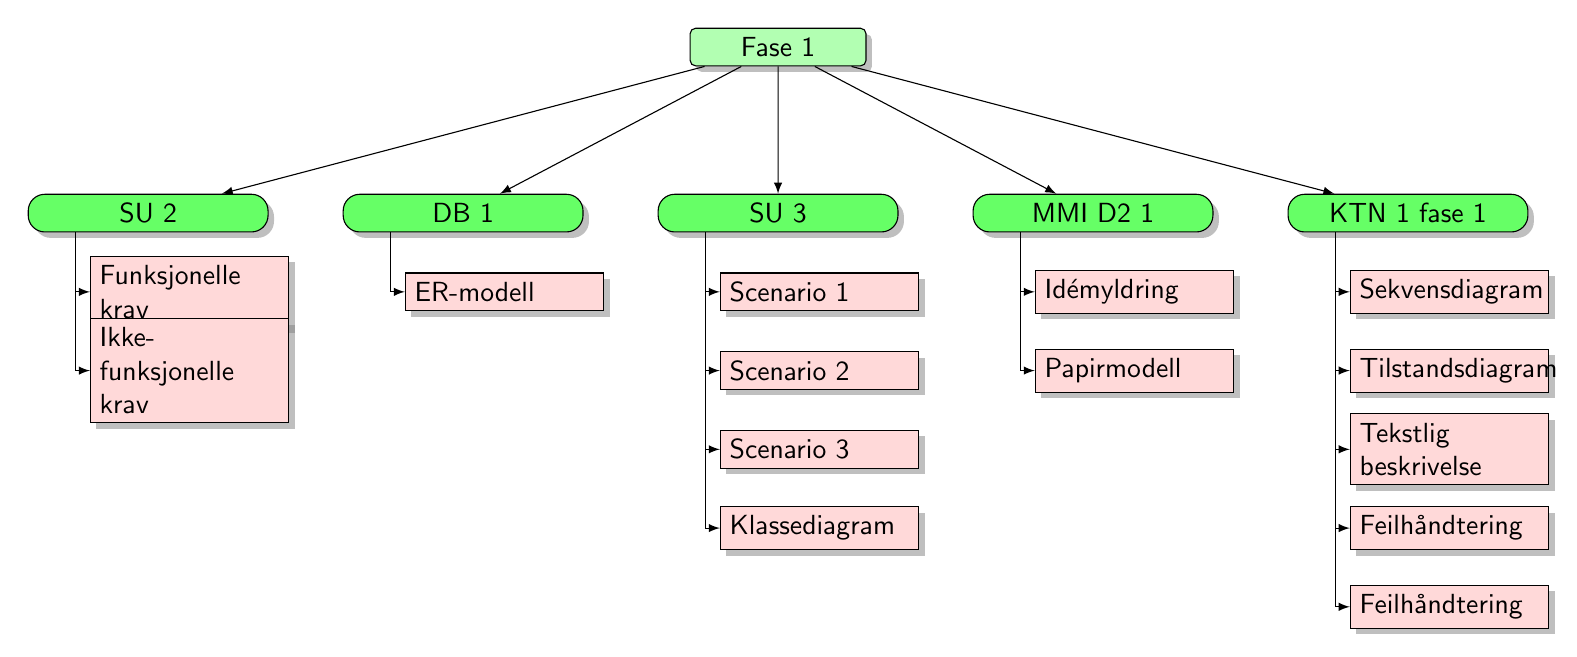
\begin{tikzpicture}[
  level 1/.style={sibling distance=40mm},
  edge from parent/.style={->,draw},
  >=latex]
  


% root of the the initial tree, level 1
\node[root] {Fase 1}
% The first level, as children of the initial tree
child {node[level 2] (c1) {SU 2}}
child {node[level 2] (c2) {DB 1}}
child {node[level 2] (c3) {SU 3}}
child {node[level 2] (c4) {MMI D2 1}}
child {node[level 2] (c5) {KTN 1 fase 1}};

% The second level, relatively positioned nodes
\begin{scope}[every node/.style={level 3}]
\node [below of = c1, xshift=15pt] (c11) {Funksjonelle krav};
\node [below of = c11] (c12) {Ikke-funksjonelle krav};

%% DB 1
\node [below of = c2, xshift=15pt] (c21) {ER-modell};

%%SU3
\node [below of = c3, xshift=15pt] (c31) {Scenario 1};
\node [below of = c31] (c32) {Scenario 2};
\node [below of = c32] (c33) {Scenario 3};
\node [below of = c33] (c34) {Klassediagram};

%%MMI D2 1
\node [below of = c4, xshift=15pt] (c41) {Idémyldring};
\node [below of = c41] (c42) {Papirmodell};

%%KTN fase 1
\node [below of = c5, xshift=15pt] (c51) {Sekvensdiagram};
\node [below of = c51] (c52) {Tilstandsdiagram};
\node [below of = c52] (c53) {Tekstlig beskrivelse};
\node [below of = c53] (c54) {Feilhåndtering};
\node [below of = c54] (c55) {Feilhåndtering};
\end{scope}
%%

% lines from each level 1 node to every one of its "children"
\foreach \value in {1,2}
  \draw[->] (c1.195) |- (c1\value.west);

\foreach \value in {1,...,1}
  \draw[->] (c2.195) |- (c2\value.west);

\foreach \value in {1,...,4}
  \draw[->] (c3.195) |- (c3\value.west);
  
\foreach \value in {1,...,2}
  \draw[->] (c4.195) |- (c4\value.west);
  
\foreach \value in {1,...,5}
  \draw[->] (c5.195) |- (c5\value.west);
\end{tikzpicture}



\end{sideways}
\newpage
\begin{sideways}
%%
%% FASE 2
%%
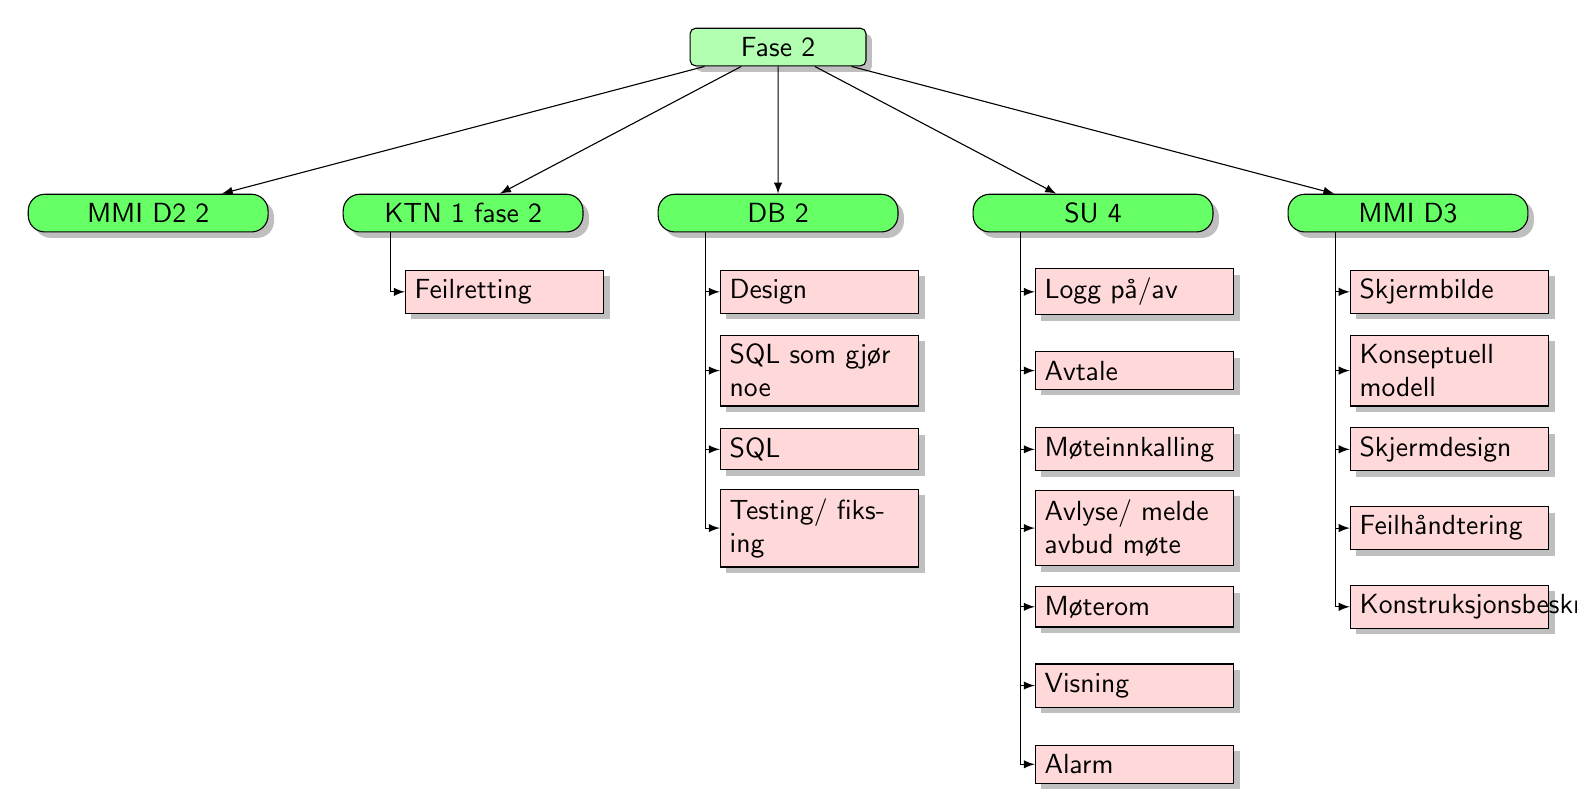
\begin{tikzpicture}[
  level 1/.style={sibling distance=40mm},
  edge from parent/.style={->,draw},
  >=latex]
  


% root of the the initial tree, level 1
\node[root] {Fase 2}
% The first level, as children of the initial tree
child {node[level 2] (c1) {MMI D2 2}}
child {node[level 2] (c2) {KTN 1 fase 2}}
child {node[level 2] (c3) {DB 2}}
child {node[level 2] (c4) {SU 4}}
child {node[level 2] (c5) {MMI D3}};


\begin{scope}[every node/.style={level 3}]
% MMI D2 2

%% KTN fase 2
\node [below of = c2, xshift=15pt] (c21) {Feilretting};

%%DB 2
\node [below of = c3, xshift=15pt] (c31) {Design};
\node [below of = c31] (c32) {SQL som gjør noe};
\node [below of = c32] (c33) {SQL};
\node [below of = c33] (c34) {Testing/ fiksing};

%%SU 4
\node [below of = c4, xshift=15pt] (c41) {Logg på/av};
\node [below of = c41] (c42) {Avtale};
\node [below of = c42] (c43) {Møteinnkalling};
\node [below of = c43] (c44) {Avlyse/ melde avbud møte};
\node [below of = c44] (c45) {Møterom};
\node [below of = c45] (c46) {Visning};
\node [below of = c46] (c47) {Alarm};

%% MMI D3
\node [below of = c5, xshift=15pt] (c51) {Skjermbilde};
\node [below of = c51] (c52) {Konseptuell modell};
\node [below of = c52] (c53) {Skjermdesign};
\node [below of = c53] (c54) {Feilhåndtering};
\node [below of = c54] (c55) {Konstruksjonsbeskrivelse};
\end{scope}
%%

% lines from each level 1 node to every one of its "children"
%\foreach \value in {0}
%  \draw[->] (c1.195) |- (c1\value.west);

\foreach \value in {1,...,1}
  \draw[->] (c2.195) |- (c2\value.west);

\foreach \value in {1,...,4}
  \draw[->] (c3.195) |- (c3\value.west);
  
\foreach \value in {1,...,7}
  \draw[->] (c4.195) |- (c4\value.west);
  
\foreach \value in {1,...,5}
  \draw[->] (c5.195) |- (c5\value.west);

\end{tikzpicture}


\end{sideways}
\newpage
\begin{sideways}
%%
%% FASE 3
%%
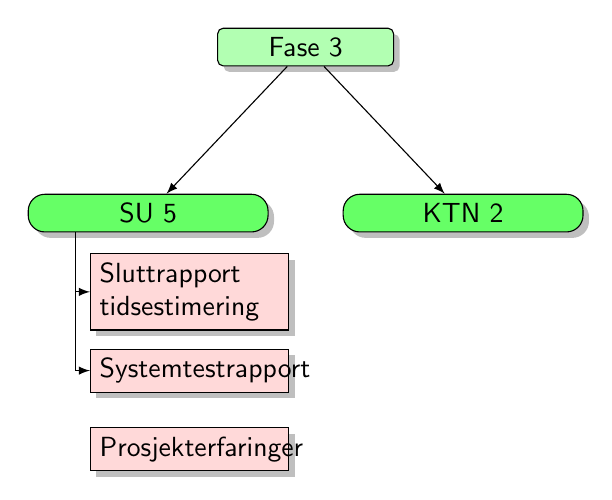
\begin{tikzpicture}[
  level 1/.style={sibling distance=40mm},
  edge from parent/.style={->,draw},
  >=latex]
  


% root of the the initial tree, level 1
\node[root] {Fase 3}
% The first level, as children of the initial tree
child {node[level 2] (c1) {SU 5}}
child {node[level 2] (c2) {KTN 2}};

% The second level, relatively positioned nodes
\begin{scope}[every node/.style={level 3}]
%% SU 5
\node [below of = c1, xshift=15pt] (c11) {Sluttrapport tidsestimering};
\node [below of = c11] (c12) {Systemtestrapport};
\node [below of = c12] (c13) {Prosjekterfaringer};
\end{scope}
%%

% lines from each level 1 node to every one of its "children"
\foreach \value in {1,2}
  \draw[->] (c1.195) |- (c1\value.west);

%\foreach \value in {1,...,1}
%  \draw[->] (c2.195) |- (c2\value.west);
\end{tikzpicture}
\end{sideways}
